\chapter{Introduction}\label{cha:intro}
\epigraph{In mesoscopic physics, you really need to build up intuition, because it is not the world you know.}{Carlo Beenakker}


\begin{figure}[!htb]
 \begin{center}
%% psfrag: comment the following line if not using the psfrag package
 % \psfrag{pie makes me happy!}{$\pi$ makes me happy!}
%% includegraphics: comment the following if not using the graphicx package
 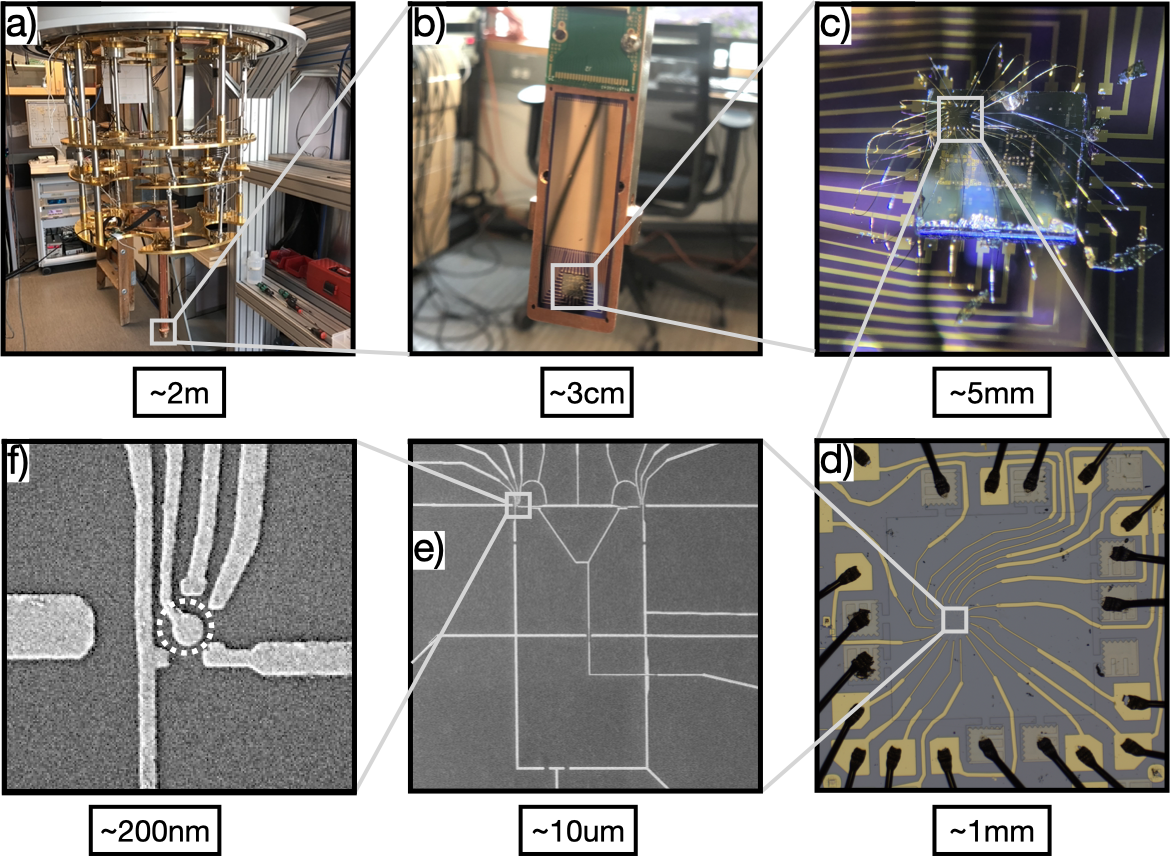
\includegraphics[width=0.95\textwidth]{figures/ch1/crop_FiguresMaster.001.png}
 \caption[Dilution fridge to quantum dot scale breakdown]{\label{fig:ch1/scale_breakdown} 
 % For some options that work with pdf\LaTeX, please see this discussion:
 % \url{http://tex.stackexchange.com/questions/11839}. 
 Illustrating the various scales to demonstrate the relationship between macroscopic changes and nanoscale effects. (\textbf{a}) Photograph of the Au-plated cold plates within a dilution refrigerator. The lowest plate, known as the mixing chamber, can reach temperatures of \qty{7}{mK}. (\textbf{b}) Photograph of the Si chip carrier, onto which the heterostructure is stuck. (\textbf{c}) Optical microscope image showing the heterostructure attached to the chip carrier. Thin Al wire bonds connect the device fabricated on the heterostructure to the fridge wires. (\textbf{d}) Optical microscope image of a single mesa on the heterostructure. A mesa is an isolated area of the heterostructure where new designs are fabricated. The black lines around the outside are wire bonds and the bright Au are thick (\qty{100}{nm}) `outer gates' which connect to the thin (\qty{10}{nm}) `inner gates'. (\textbf{e}) Scanning electron micrograph (SEM) of the inner gates. The mean free path of the electrons is of order \qty{3}{\mu m}. (\textbf{f}) SEM image zooming in on the quantum dot. By carefully tuning the voltages on the inner gates, an isolated puddle of electrons is engineered, typically with a total occupation of 0 - 10. 
  }
 \end{center}
\end{figure}




Mesoscopic physics is a discipline situated within the domain of condensed matter physics and between the dimensions of nanometer to micrometer. Mesoscopic systems unveil a rich zoo of quantum phenomena and material properties. 
Distinct from their macroscopic counterparts, mesoscopic systems can exhibit behavior influenced by quantum effects. One of the initial measurements of a mesoscopic system studied the conductance through a quantum wire~\cite{qpc_first_measurement, qpc_second_measurement}. 
Classically, we expect conductance to be proportional to the width of the wire. 
However, a quantum wire exhibits steps at integer values of conductance as the width is varied. 
Another milestone in the field was the discovery of Coulomb blockade oscillations in the conductance measured across a quantum dot ~\cite{first_charging_of_qd}. 
In this experiment, a small isolated island of electrons was connected to two baths of electrons through tunnel barriers. 
The island's small size resulted in charge quantisation and significant spacing between orbital energy levels, effectively forming an `artificial atom'. 
The benefits of this system come from a high degree of tunability and control. Where the relevant scales that allow human control over this `artificial atom' are illustrated in Fig.~\ref{fig:ch1/scale_breakdown}.
The scope of mesoscopic physics is continually expanding, with ongoing developments in new materials~\cite{manfra_inas}, measurement methods~\cite{child_meas}, and arrangement of systems~\cite{borsoi2022shared, raysu}.

Theorists and experimentalists enjoy a symbiotic relationship in mesoscopic physics. Experiments serve to validate established theories, while theorists are tasked with modeling surprising and repeatable phenomena discovered in experiments. Notable examples of successful experiments validating theory include the investigation of Wigner crystals~\cite{wigner_solid}, isolation of graphene~\cite{graphene}, and measurement of quasiparticle charge in fractional quantum Hall~\cite{fractional_charge}. Conversely, instances of unexpected experimental findings that prompted theoretical inquiry include integer quantum Hall effect~\cite{klitzing}, anomalous Landau quantisation~\cite{landau_quantisation}, and superconductivity in twisted double bilayer graphene~\cite{raysu}.

The focus of this thesis centers on a phenomenon initially discovered through experimental observation, subsequently prompting theorists to develop a new model capable of predicting the striking behavior observed in measurements. The Kondo effect, first discovered in impure bulk metals in the 1930s~\cite{de_haas} and explained later in the 1960s~\cite{jun_kondo}, has seen significant interest in the field of quantum devices. The high degree of tunability and control in these devices allows for testing theoretical predictions ~\cite{costi_kondo_mv_eo_regime}. 
The Kondo effect in quantum devices involves a net spin (odd number of electrons) in a quantum dot, strongly coupled to two electron reservoirs. Virtual tunnel events through the quantum dot, with possible spin flips lead to a correlated state, the Kondo singlet. The Kondo effect can be seen in the enhanced conductance, with decreasing temperature, in between Coulomb blockade peaks. This conductance approaches the unitary limit, where the transmission probability through the quantum dot is one~\cite{kondo_unitary, kondo_unitary_theory, yigal_kondo}. A remarkable effect as the tunnel barriers into the quantum dot each have a transmission probability of less than one. More recent experiments have explored exotic regimes of the Kondo effect, Kondo effect in graphene~\cite{kondo_graphene}, Kondo lattices are used to study quantum criticality~\cite{kondolattice}, multi-channel Kondo has been observed, and can lead to non-Fermi liquid
behaviour~\cite{potok_2ck, iftikhar_2ck, kirchner_2ck} and the novel topological Kondo effect which could demonstrate the non-local quantum dynamics of Majorana fermions~\cite{topological_kondo_majorana, topological_kondo, kondo_topological}.

Nevertheless, there remains considerable potential for further insights by extending the scope of the initial, seemingly 'simple' measurements on the Kondo effect into new parameter regimes. In this thesis, we develop and test a novel method for measuring the Kondo effect with weaker coupling than previously explored.


